%\documentclass{beamer}%[aspectratio=169]
\documentclass[aspectratio=169,mathserif]{beamer}  %[aspectratio=169]

% \usepackage{pgfpages} 
% \setbeameroption{show notes on second screen} 
%
% Choose how your presentation looks.
%
% For more themes, color themes and font themes, see:
% http://deic.uab.es/~iblanes/beamer_gallery/index_by_theme.html

%\mode<presentation>
%{
\usecolortheme{ruc} % or try albatross, beaver, crane, ...
%\usefonttheme{professionalfonts}  
\usefonttheme{serif} % default family is serif
\usepackage{fontspec}
%\setmainfont{Bitstream Vera Serif}
%\setmainfont{EB Garamond}
%\setmainfont{Baskerville}
\setmainfont{Georgia}
\setbeamertemplate{navigation symbols}{}
\setbeamertemplate{caption}[numbered]
\setbeamertemplate{footline}[frame number]
%} 
\usepackage[english]{babel}
\usepackage[utf8x]{inputenc}
\usepackage{subfigure}
\usepackage{color}
\usepackage{bm}
\usepackage{multirow}
\usepackage[absolute,overlay]{textpos}
  \setlength{\TPHorizModule}{1mm}
  \setlength{\TPVertModule}{1mm}

\usepackage{pgfpages}
% These slides also contain speaker notes. You can print just the slides,
% just the notes, or both, depending on the setting below. Comment out the want
% you want.
\setbeameroption{hide notes} % Only slides
%\setbeameroption{show only notes} % Only notes
%\setbeameroption{show notes on second screen=right} % Both  

\usepackage{amsmath}
\usepackage{amssymb}
\usepackage{amsfonts}
\usepackage{bm}
\usepackage{graphicx}
\usepackage{cancel}

\usepackage[backend=bibtex,sorting=none]{biblatex}
\addbibresource{references.bib}
\setbeamerfont{footnote}{size=\tiny}
\setbeamertemplate{bibliography item}[text]
\newcommand{\dd}{\mathrm{d}}
\newcommand{\R}{\mathbb{R}}
\newcommand{\E}{\mathbb{E}}
\newcommand{\light}[1]{\textcolor{gray}{#1}}
\newcommand{\tb}{\textbf}
\newcommand{\red}{\textcolor{red}}


\title[12.23Pre]{\huge{\textbf{Equivariant Subgraph Aggregation Networks}}}
\author{Beatrice Bevilacqua \quad Fabrizio Frasca \quad Derek Lim \quad Balasubramaniam~Srinivasan \quad Chen Cai \quad Gopinath Balamurugan \quad Michael~M. Bronstein \quad Haggai Maron\\
\tb{presenter}: Shen Yuan
}
\date{}


\begin{document} 


\begin{frame}
  \titlepage
  \vspace{-1cm}
  \centering
  \includegraphics[width=0.4\linewidth]{ruc_logo.png}\quad
  \includegraphics[width=0.4\linewidth]{GSAI_logo.png}
\end{frame}



\begin{frame}[noframenumbering]
\begin{itemize}
    \begin{LARGE}
    \item Introduction
    \item \light{Equivariant Subgraph Aggregation Networks(ESAN)}
    \item \light{A WL Analogue for ESAN}
    \item \light{Experiments}
    \item \light{Summary}
    \end{LARGE}
\end{itemize}
\end{frame}



\begin{frame}{Preliminary}

\tb{Graph Isomorphism} Two graphs are considered isomorphic if there is a mapping between the nodes of the graphs that preserves node adjacencies.

\begin{figure}[t]
\centerline{\includegraphics[width=0.7\linewidth]{figure5.png}}
\end{figure}

\end{frame}



\begin{frame}{Preliminary}

\tb{1-dimensional Weisfeiler-Leman (1-WL) test} 
It's a simple iterative algorithm to distinguish two graphs, which can produce for each graph a canonical form. 

\pause
\begin{itemize}[<+->]
    \item If the canonical forms of two graphs are \tb{not equivalent}, then the graphs are definitively not isomorphic. 
    \item If the canonical forms of two graphs are \tb{equivalent}, the graphs may be isomorphic. 
\end{itemize}

\end{frame}





\begin{frame}{Test!}

\tb{Are these two graphs isomorphic?}

\begin{figure}[t]
\centerline{\includegraphics[width=0.7\linewidth]{figure9.png}}
\end{figure}

\end{frame}



\begin{frame}{Test!}

\tb{Are these two graphs isomorphic? YES!}

\begin{figure}[t]
\centerline{\includegraphics[width=0.7\linewidth]{figure9.png}}
\end{figure}

\end{frame}



\begin{frame}{1-dimensional Weisfeiler-Leman (1-WL) Test}

\begin{figure}[t]
\centerline{\includegraphics[width=0.5\linewidth]{figure9.png}}
\end{figure}

\begin{eqnarray*}
\begin{aligned}
c_{v}^{t+1} \gets \text{HASH}(c_{v}^{t}, N_{v}^{t})
\end{aligned}    
\end{eqnarray*}

\end{frame}



\begin{frame}{Motivation}

While two graphs may not be distinguishable by 1-WL test, they often contain distinguishable subgraphs. 

\pause 

\begin{figure}[t]
\centerline{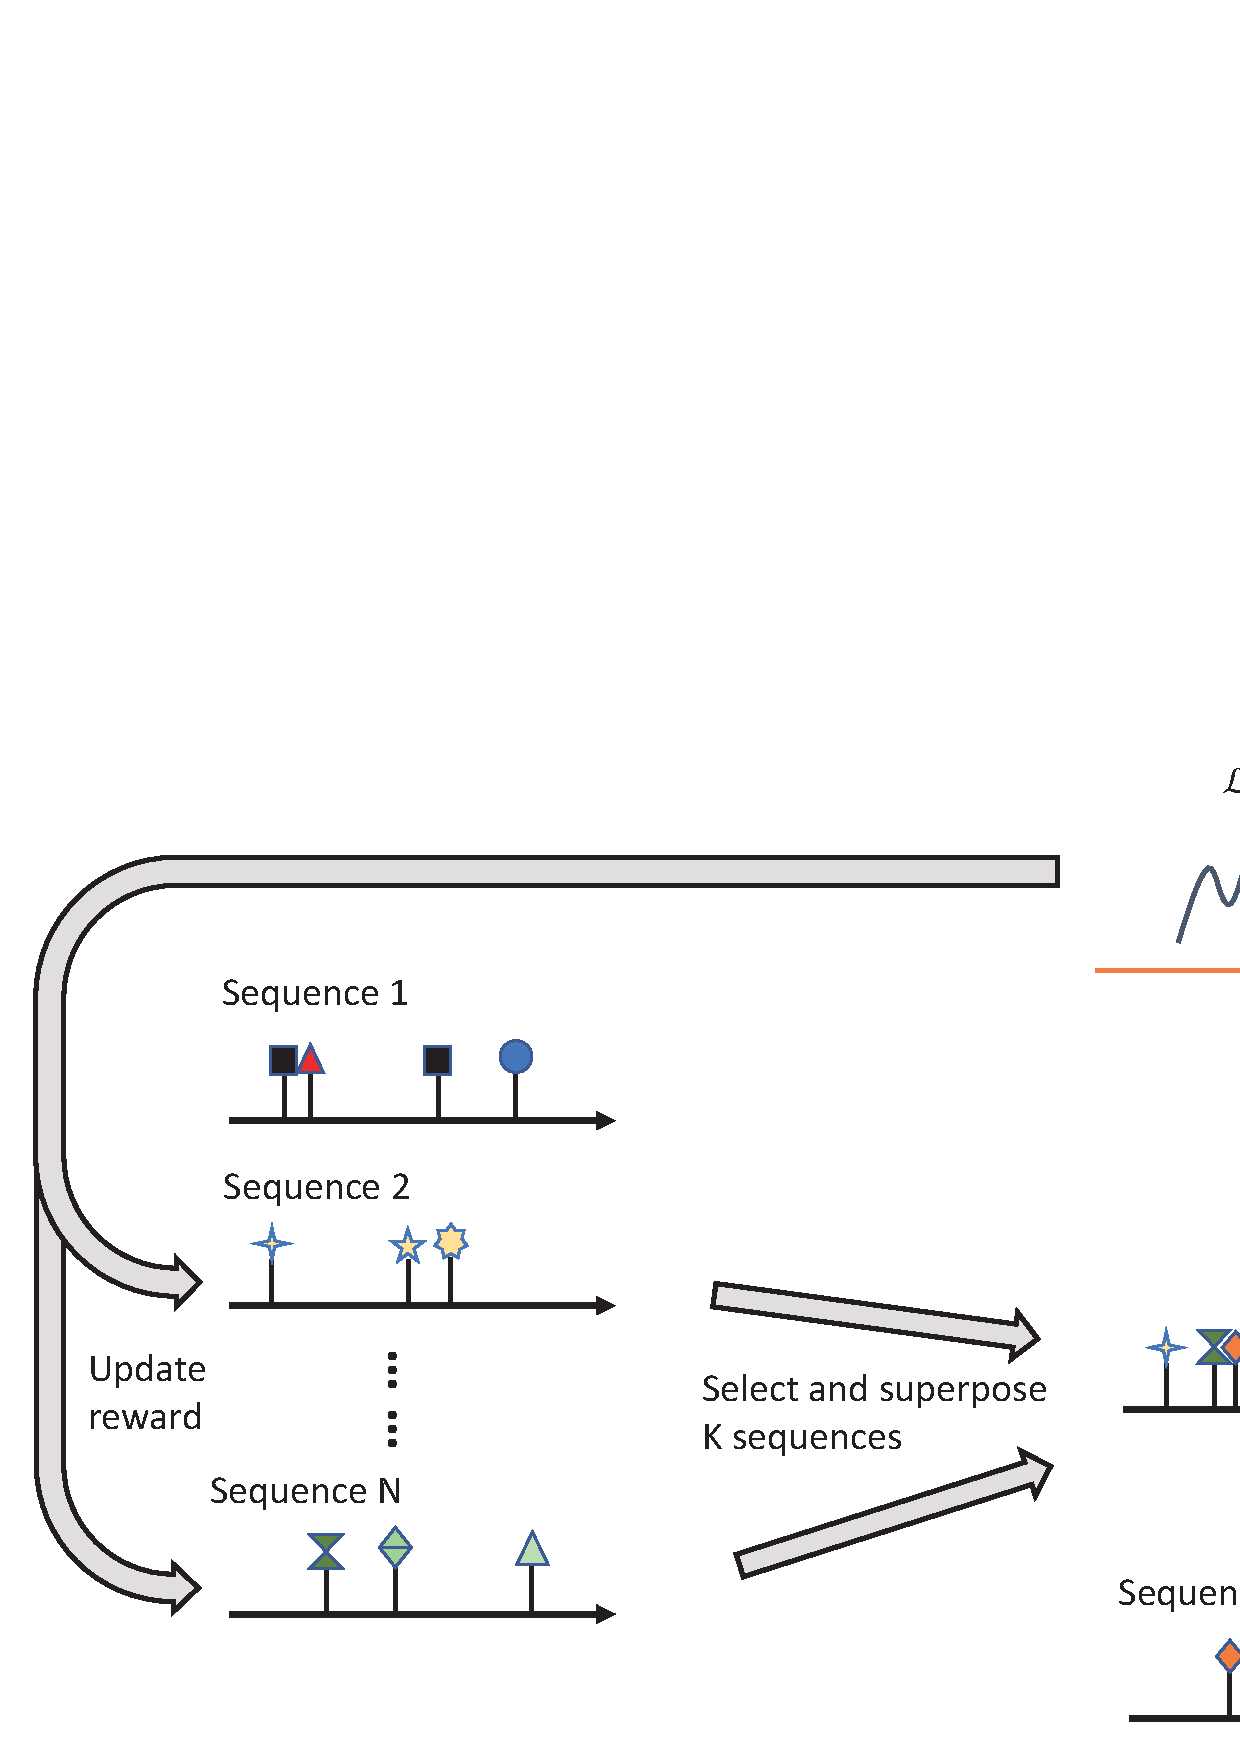
\includegraphics[width=0.7\linewidth]{figure1.png}}
\label{fig1}
\end{figure}

\end{frame}



\begin{frame}{Contribution}

\begin{itemize}
    \item This paper proposed a framework called \tb{Equivariant Subgraph Aggregation Networks(ESAN)} to improve expressive power of MPNNs.
    \item It developed variants \tb{DS(S)-WL} of \tb{the 1-dimensional Weisfeiler-Leman (1-WL) test} for graph isomorphism.
\end{itemize}

\end{frame}



\begin{frame}[noframenumbering]
\begin{itemize}
    \begin{LARGE}
    \item \light{Introduction}
    \item Equivariant Subgraph Aggregation Networks(ESAN)
    \item \light{A WL Analogue for ESAN}
    \item \light{Experiments}
    \item \light{Summary}
    \end{LARGE}
\end{itemize}
\end{frame}



\begin{frame}{Equivariant Subgraph Aggregation Networks(ESAN)}

The ESAN framework consists of 
\begin{itemize}[<+->]
    \item Neural network architectures for processing bags of subgraphs (\tb{DSS-GNN} and \tb{DS-GNN})
    \item Subgraph selection policies
\end{itemize}

\end{frame}



\begin{frame}{DSS-GNN}

\begin{figure}[t]
\centerline{\includegraphics[width=0.9\linewidth]{figure3.png}}
\end{figure}

\end{frame}


\begin{frame}{Bags-of-Graphs Encoder Architecture}

\begin{columns}[T]
\begin{column}{0.55\textwidth}
\begin{itemize}[<+->]
    \item The bag(multiset) $S_G=\{G_1,\ldots,G_m\}$ of subgraphs of $G$ can be represented as tensor $(\mathcal{A, X})\in \R^{n\times n \times m}\times \R^{n\times d\times m}$ 
    \item $n$ denotes the number of nodes and $m$ the number of subgraphs
    \item $\mathcal{A}\in\R^{n\times n \times m}$ represents a set of m adjacency matrices, and $\mathcal{X}\in\R^{n\times d \times m}$ represents a set of $m$ node feature matrices. 
    \item $\sigma\in S_n$ means node permutations, $(\sigma\cdot A)_{ij}=A_{\sigma^{-1}(i)\sigma^{-1}(j)},\ (\sigma\cdot X)_{il}=X_{\sigma^{-1}(i)l}$
    $\tau\in S_m$ means subgraph permutations, $(\tau\cdot \mathcal{A})_{ijk}=\mathcal{A}_{ij\tau^{-1}(k)},\ (\tau\cdot \mathcal{X})_{ilk}=\mathcal{X}_{il\tau^{-1}(k)}$
\end{itemize}
\end{column}
\begin{column}{0.4\textwidth}
    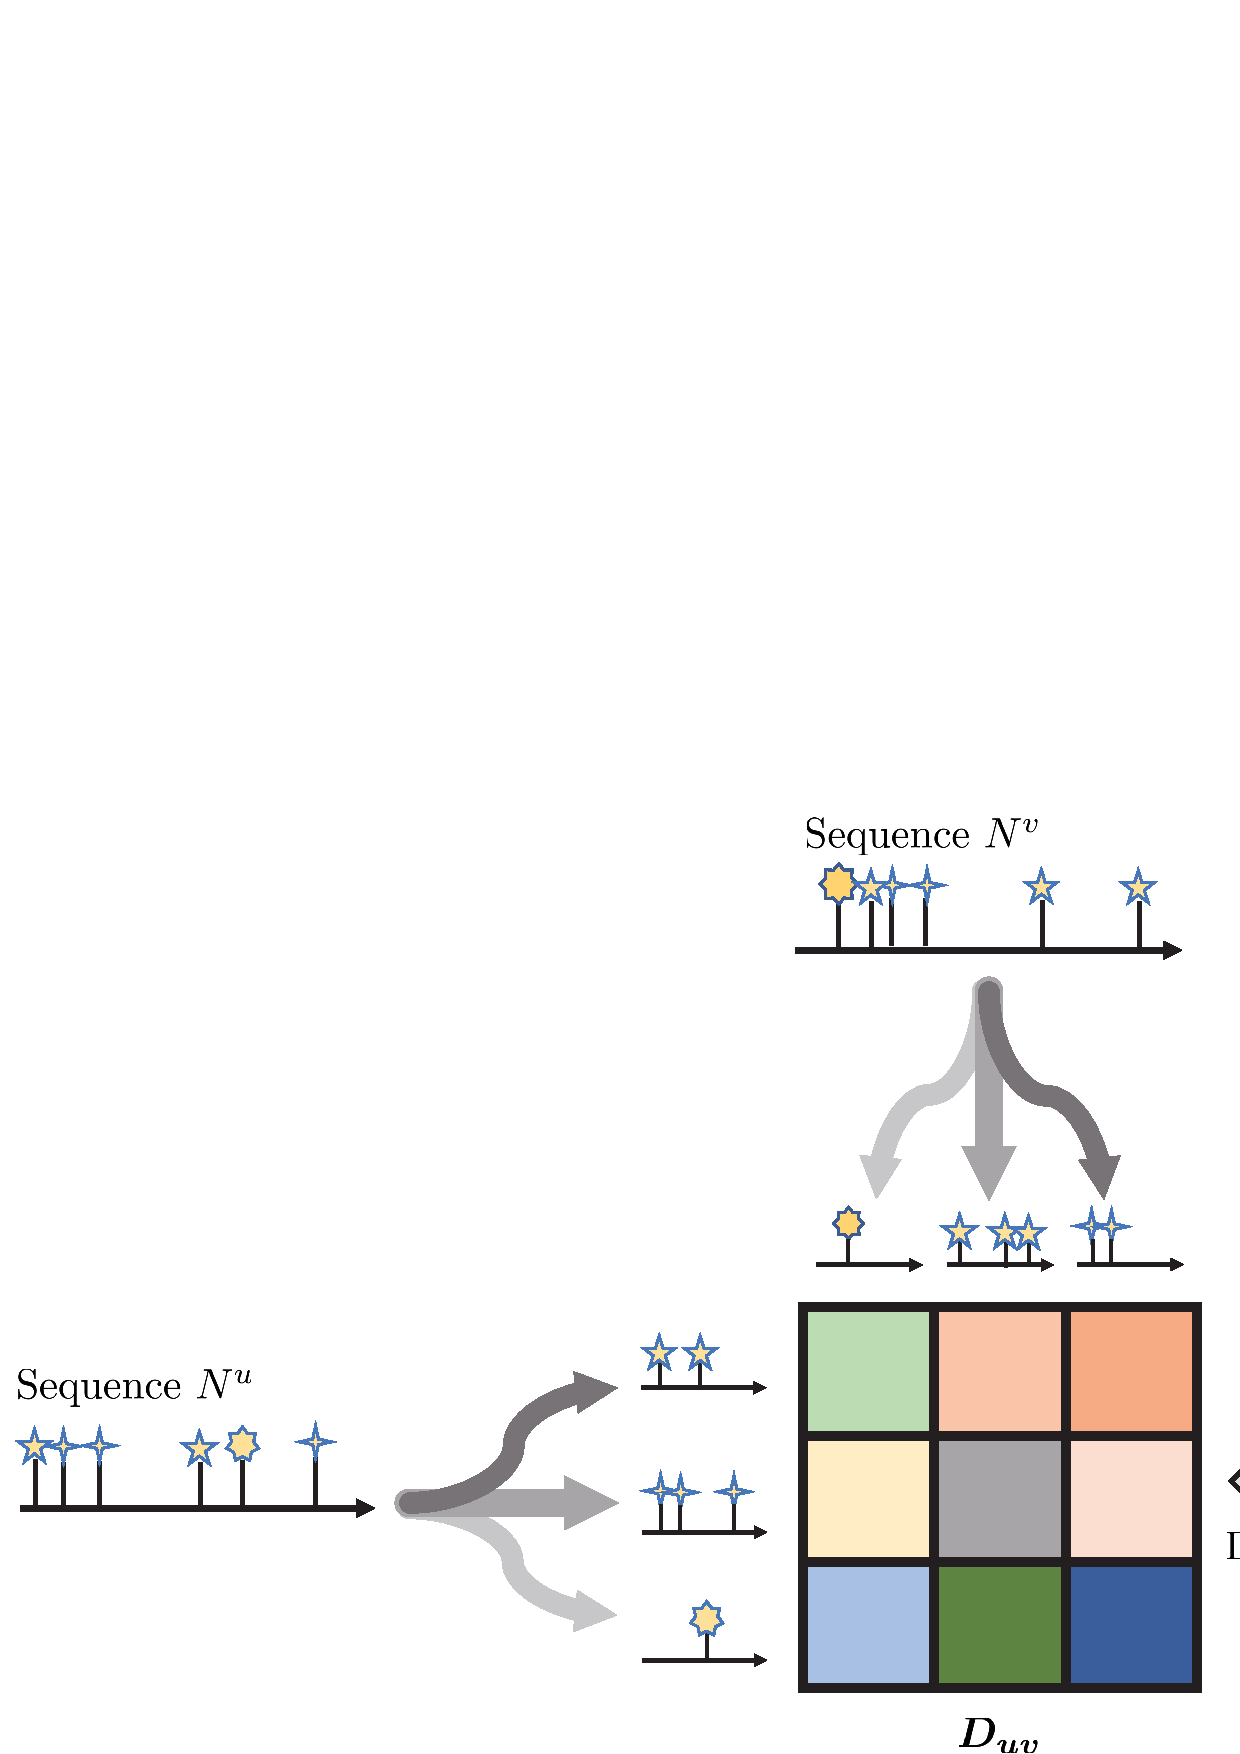
\includegraphics[width=\linewidth]{figure2.png}
\end{column}
\end{columns}

\end{frame}



\begin{frame}{H-equivariant layers}

\begin{columns}[T]
\begin{column}{0.55\textwidth}
\begin{itemize}[<+->]
    \item $L:\R^{n\times n \times m}\times \R^{n\times d\times m} \to \R^{n\times n \times m}\times \R^{n\times d' \times m}$ map bags of subgraphs to bags of subgraphs:
    \item 
        \begin{eqnarray*}
        \begin{aligned}
        (L(\mathcal{A,X}))_i=L^1(\mathcal{A}_i,\mathcal{X}_i)+L^2(\sum_{j=1}^{m}A_j,\sum_{j=1}^{m}X_j)
        \end{aligned}    
        \end{eqnarray*}
    \item $L^1,L^2:\R^{n\times n}\times \R^{n\times d}\to \R^{n\times n}\times \R^{n\times d'}$ represent two graph encoders and can be any type of GNN layer. 
\end{itemize}
\end{column}
\begin{column}{0.4\textwidth}
    \includegraphics[width=\linewidth]{figure6.png}
\end{column}
\end{columns}

\end{frame}



\begin{frame}{Subgraph Selection Policies}

This paper explores four simple subgraph selection policies: 
\begin{itemize}[<+->]
    \item The \tb{node-deleted policy(ND)}, a graph is mapped to the set containing all subgraphs that can be obtained from the original graph by removing a single node
    \item The \tb{edge-deleted policy(ED)} is defined by removing a single edge
    \item The \tb{ego-networks policy(EGO)} maps each graph to a set of ego-networks of some specified depth, one for each node in the graph (a k-Ego-network of a node is its k-hop neighbourhood with the induced connectivity).
    \item The \tb{EGO+} is a variant of the \tb{EGO} where the root node holds an identifying feature
\end{itemize}

\end{frame}



\begin{frame}[noframenumbering]
\begin{itemize}
    \begin{LARGE}
    \item \light{Introduction}
    \item \light{Equivariant Subgraph Aggregation Networks(ESAN)}
    \item A WL Analogue for ESAN
    \item \light{Experiments}
    \item \light{Summary}
    \end{LARGE}
\end{itemize}
\end{frame}



\begin{frame}{DSS-WL and DS-WL}

This paper proposed DSS-WL and DS-WL that are variants of 1-WL test.
The only difference is \tb{refinement} step.

\begin{eqnarray*}
\begin{aligned}
c_{v,S}^{t+1} \gets \text{HASH}(c_{v,S}^{t}, N_{v,S}^{t}, C_{v}^{t}, M_{v}^{t})
\end{aligned}    
\end{eqnarray*}

\begin{itemize}
    \item $N_{v,S}^{t}$ denotes the multiset of colors in $v$’s neighborhood over subgraph $S$
    \item $C_{v}^{t}$ represents the multiset of v’s colors across subgraphs
    \item $M_{v}^{t}$ denotes the multiset of colors in $v$’s neighborhood over original graph $G$
\end{itemize}

\pause

\tb{Is DS(S)-WL strictly more powerful than 1-WL?}

\end{frame}



\begin{frame}{Circulant Skip Link(CSL)}

CSL($n,2$) can be distinguished from any CSL($n,k$) with $k\in[3,n/2-1]$ by DS-WL and DSS-WL with either the ND, EGO, or EGO+ policy.

\begin{figure}[t]
\centerline{\includegraphics[width=0.9\linewidth]{figure4.png}}
\end{figure}
    
\end{frame}



\begin{frame}[noframenumbering]
\begin{itemize}
    \begin{LARGE}
    \item \light{Introduction}
    \item \light{Equivariant Subgraph Aggregation Networks(ESAN)}
    \item \light{A WL Analogue for ESAN}
    \item Experiments
    \item \light{Summary}
    \end{LARGE}
\end{itemize}
\end{frame}



\begin{frame}{Experiments}

\begin{figure}[t]
\centerline{\includegraphics[width=0.68\linewidth]{figure7.png}}
\end{figure}

\end{frame}



\begin{frame}{Experiments}

\begin{figure}[t]
\centerline{\includegraphics[width=0.45\linewidth]{figure8.png}}
\end{figure}

\end{frame}



\begin{frame}[noframenumbering]
\begin{itemize}
    \begin{LARGE}
    \item \light{Introduction}
    \item \light{Equivariant Subgraph Aggregation Networks(ESAN)}
    \item \light{A WL Analogue for ESAN}
    \item \light{Experiments}
    \item Summary
    \end{LARGE}
\end{itemize}
\end{frame}



\begin{frame}{Summary}

\begin{itemize}[<+->]
    \item The core idea is to learn the subgraphs set instead of original graph.
    \item The DSS-GNN framework take 3x the time of the corresponding base graph encoder to obtain a little promotion.
\end{itemize}

\end{frame}



\end{document}	% Done!

